\section{Frequency mode 13}
\label{sec:fm13}

\subsection{Overview}
\label{sec:fm13:overview}
Frequency mode~13 monitors the band $556.598$--$557.398\,\mathrm{GHz}$. Its
main use is retrievals of \chem{H_2O} and \chem{O_3}.
This is the strongest water vapour line available in the sub-mm wave spectrum
and is used to reach the  highest possible altitude particularly to study
water vapour around the mesopause region.  The line centre is saturated up to
approximately 90~km and therefore temperatures can be derived throughout the
mesosphere. This band and FM~19 remain problematic and require a dedicated
study to understand the presumably instrumental effects.
Spectra from this observation mode are shown in Figure~\ref{fig:spectra:13}.

\begin{figure}[ht]
    \centering
    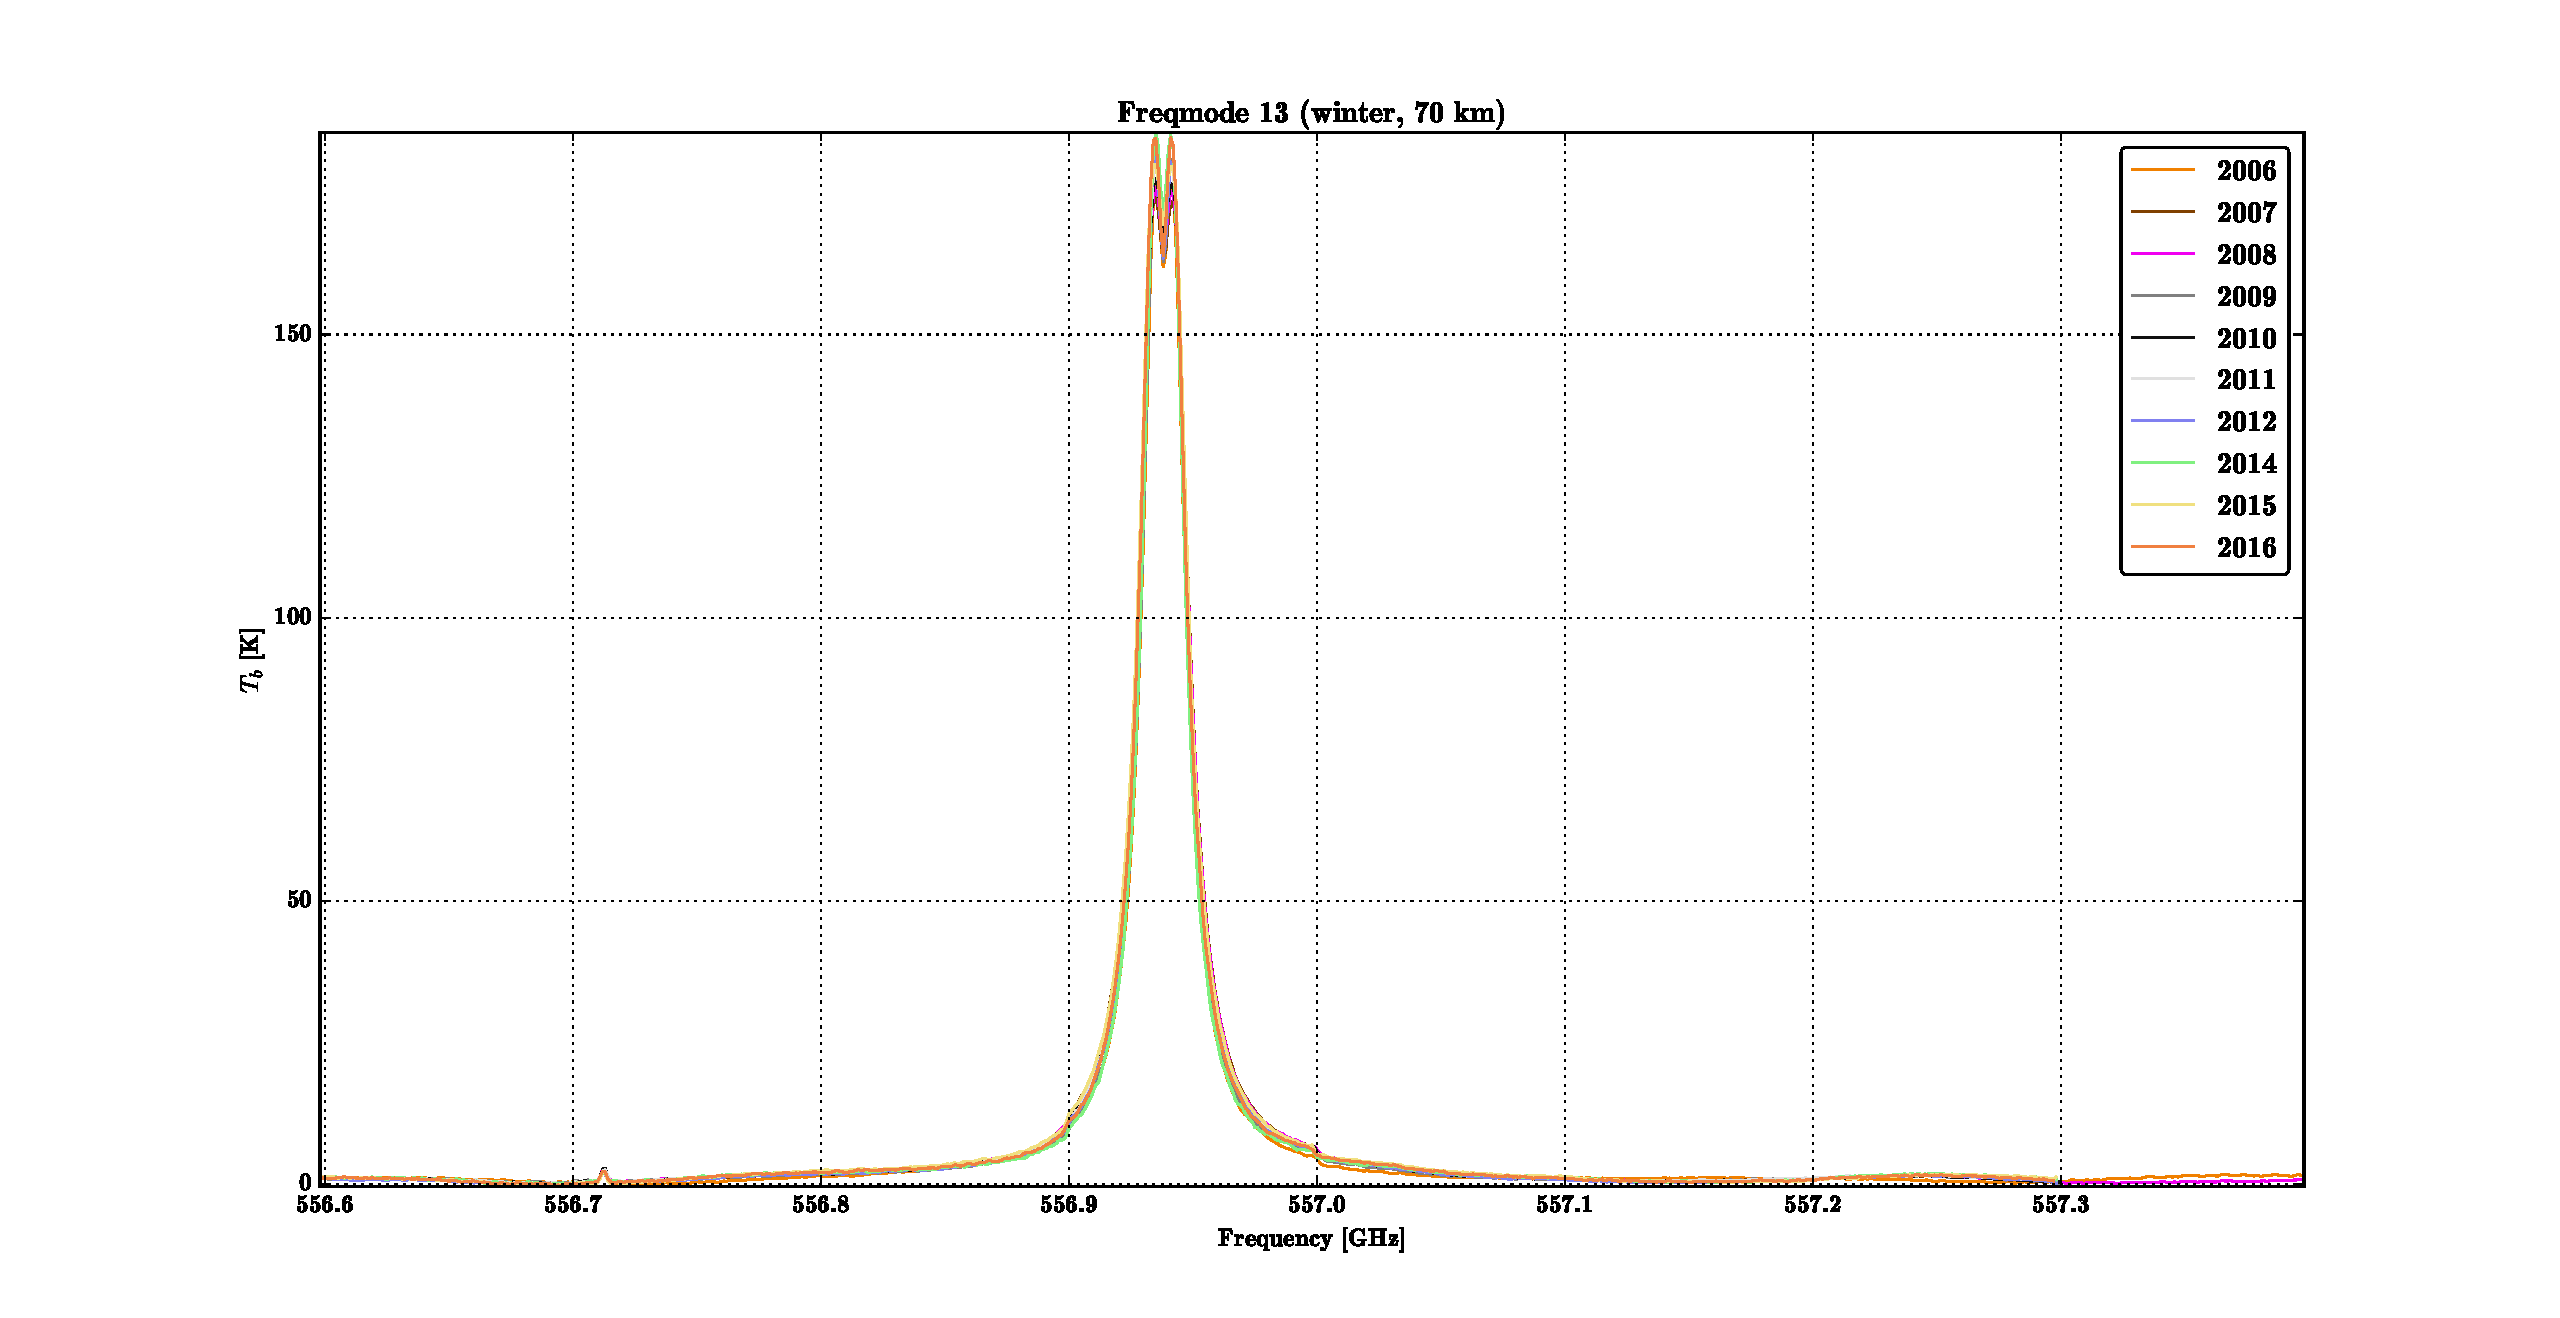
\includegraphics[width=0.95\textwidth]{spectra/fm_13_spectra_winter}
    \caption{Annual median spectra for FM~13 for altitude interval 65--75~km at
        equatorial latitudes during the arctic winter.
    }\label{fig:spectra:13}
\end{figure}


\subsection{Comparison of retrieved profiles}
\label{sec:fm13:comparison}


%%%%%%
% O3 %
%%%%%%

\subsubsection{\chem{O_3}}
\label{sec:fm13:comparison:O3}
The retrievals for \chem{O_3} have been compared with data from the MIPAS, MLS
and OSIRIS instruments. Annual average differences to these instruments are
shown in Figure~\ref{fig:fm13:O3:profiles}. In Figure~\ref{fig:fm13:O3:scatter}
individual retrievals for the instruments for the entire period are plotted
against the retrievals from the new and old versions of the \smr\ processing
chain. The results show a better overall coherency with the updated version
of the processing compared to all considered instruments, but a systematic
under estimation of the concentrations has been introduced. The reason for this
is that a previously introduced  (ver 2.1) empirical correction to the intensities has been remove since there
was no physical basis for its inclusion. We suspect that some sort of
non-linearity is causing the underestimation. Investigations of this band are continuing. 
Above about 65 km diurnal variability in the ozone concentration introduce problems when comparing with instruments
on different platforms.   We assume that this is the main reason for the differences at such altitudes. 
Figure~\ref{fig:fm13:O3:mr_avk}
suggests that the product is useful over the range 44--80~km with a vertical
resolution of around 6~km.


\begin{figure}[tbhp]
    \centering
    \begin{subfigure}[b]{0.49\textwidth}
        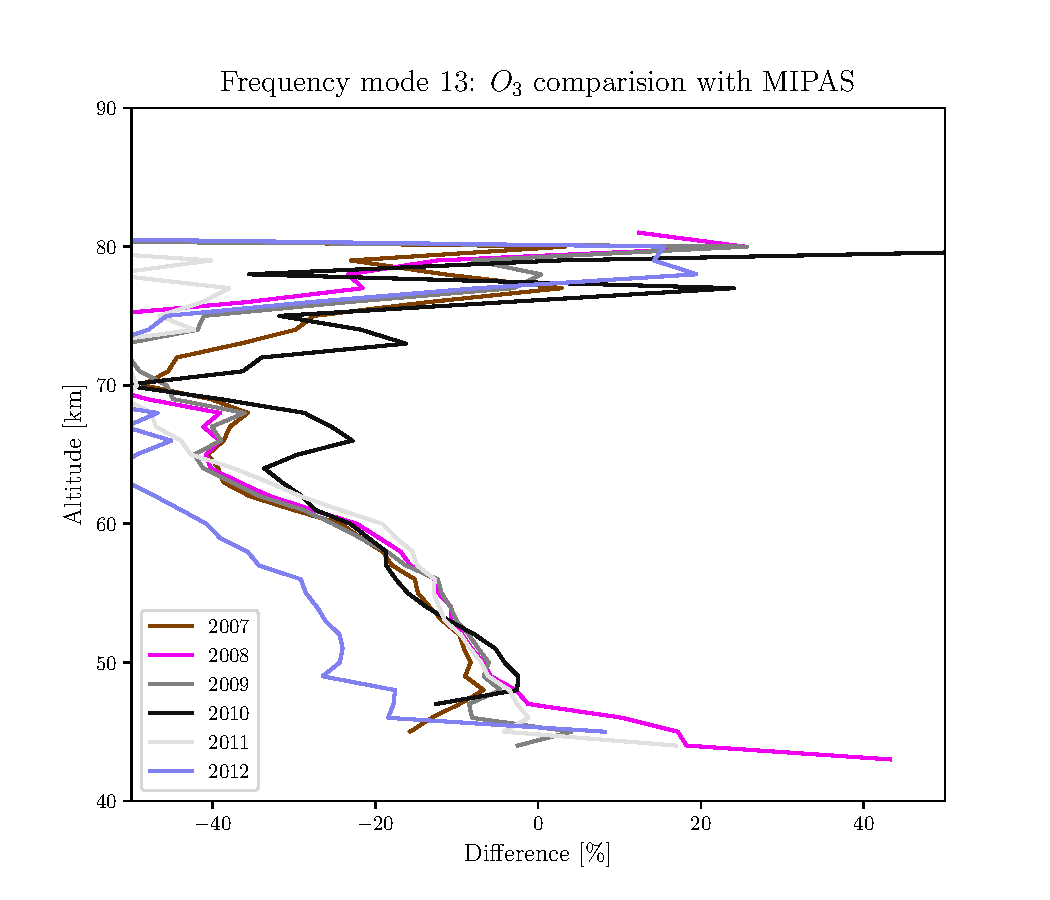
\includegraphics[width=\textwidth]{DDS_fm13_O3_perdiff_mipas}
        \caption{average difference to MIPAS}
        \label{fig:fm13:O3:profiles:MIPAS}
    \end{subfigure}
    \,
    \begin{subfigure}[b]{0.49\textwidth}
        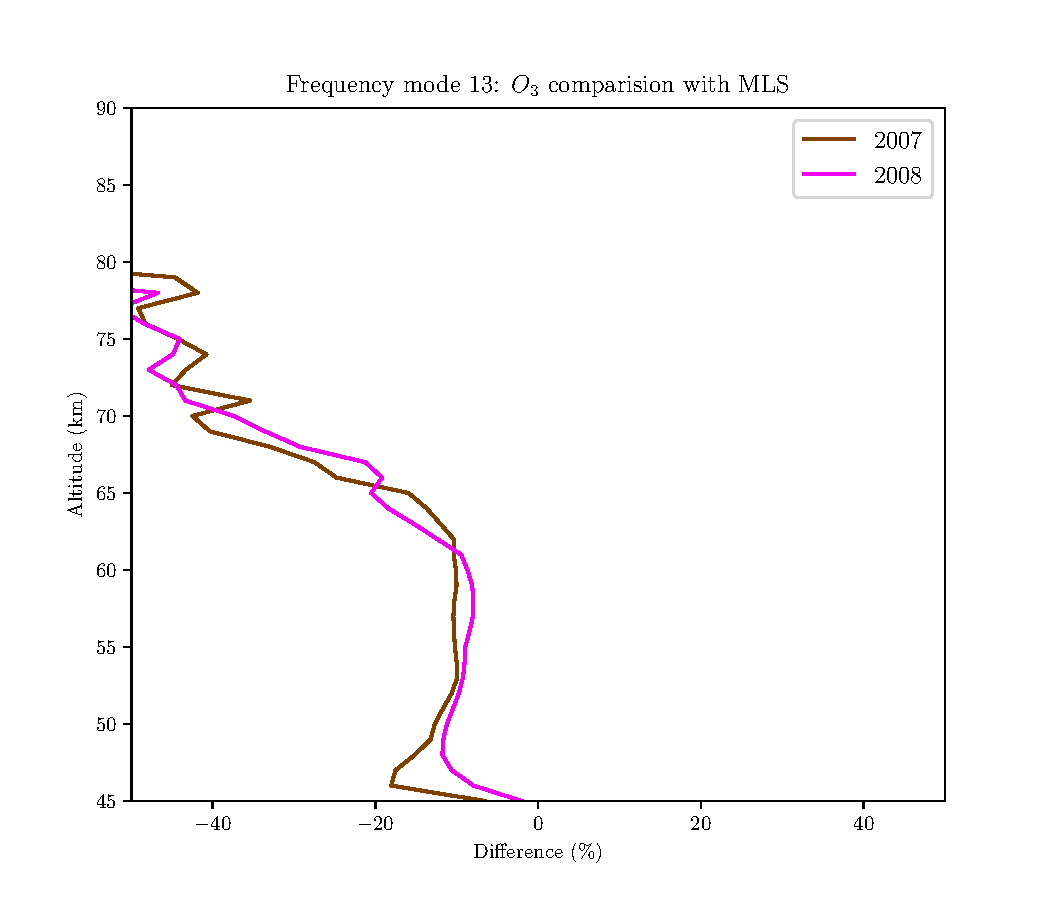
\includegraphics[width=\textwidth]{DDS_fm13_O3_perdiff_mls}
        \caption{average difference to MLS}
        \label{fig:fm13:O3:profiles:MLS}
    \end{subfigure}

    \begin{subfigure}[b]{0.49\textwidth}
        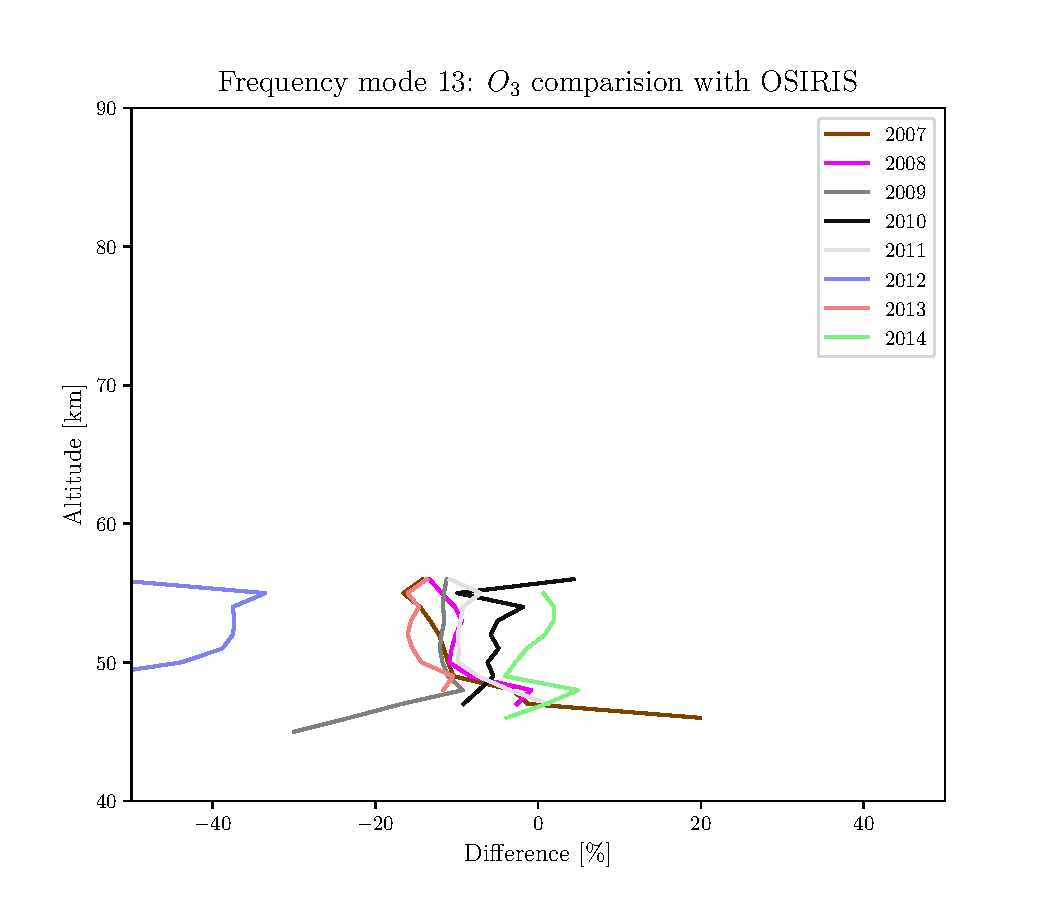
\includegraphics[width=\textwidth]{DDS_fm13_O3_perdiff_osiris}
        \caption{average difference to OSIRIS}
        \label{fig:fm13:O3:profiles:OSIRIS}
    \end{subfigure}
    \caption{Average difference in percent between retrievals of \chem{O_3}
    from \smr~v3 and collocated measurements from various instruments at
    different altitudes for frequency mode~13.}

    \label{fig:fm13:O3:profiles}
\end{figure}

\begin{figure}[tbhp]
    \centering
    \begin{subfigure}[b]{0.49\textwidth}
        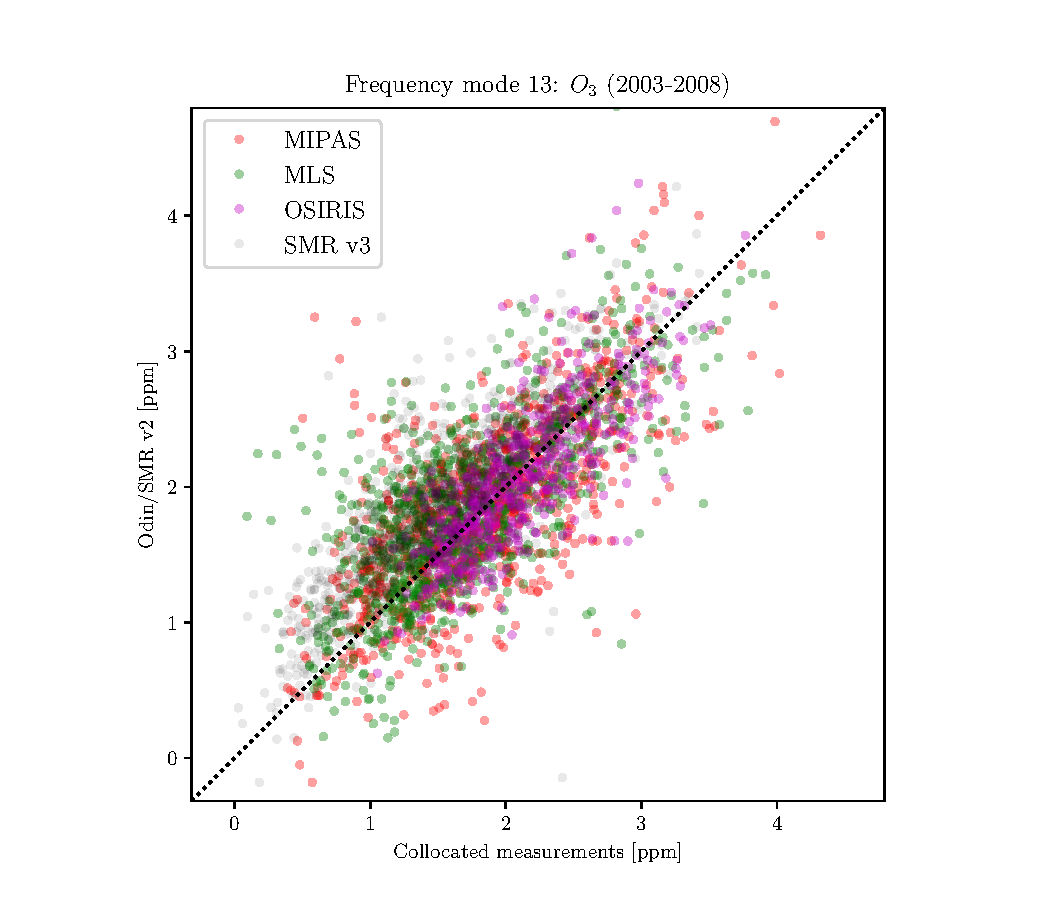
\includegraphics[width=\textwidth]{DDS_fm13_O3_scatter_v2}
        \caption{correlation of collcated instruments with \smr~v2.X}
        \label{fig:fm13:O3:scatter:v2}
    \end{subfigure}
    \,
    \begin{subfigure}[b]{0.49\textwidth}
        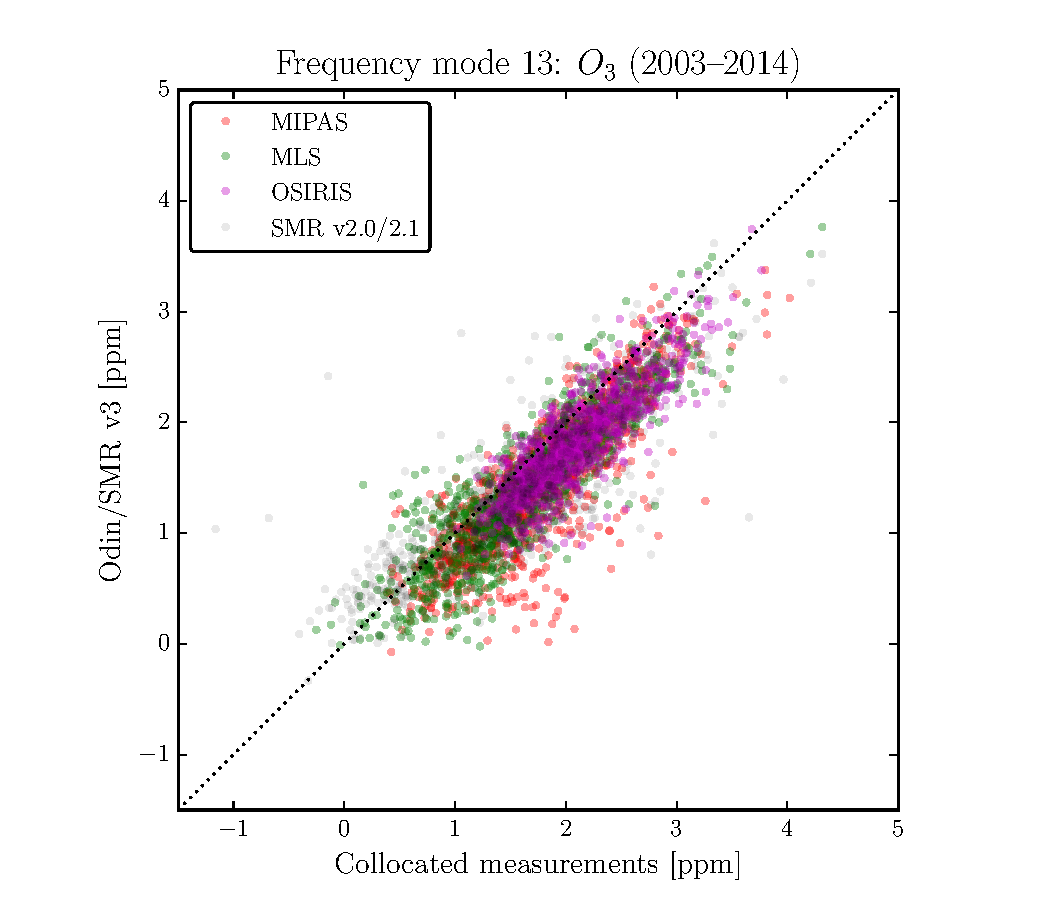
\includegraphics[width=\textwidth]{DDS_fm13_O3_scatter_v3}
        \caption{correlation of collcated instruments with \smr~v3}
        \label{fig:fm13:O3:scatter:v3}
    \end{subfigure}
    \caption{Correlation between retrievals of \chem{O_3} using \smr\
    versions~2.X and~3 and collocated measurements from various instruments
    for frequency mode~13.}
    \label{fig:fm13:O3:scatter}
\end{figure}

\begin{figure}[tbhp]
    \centering
    \begin{subfigure}[b]{0.49\textwidth}
        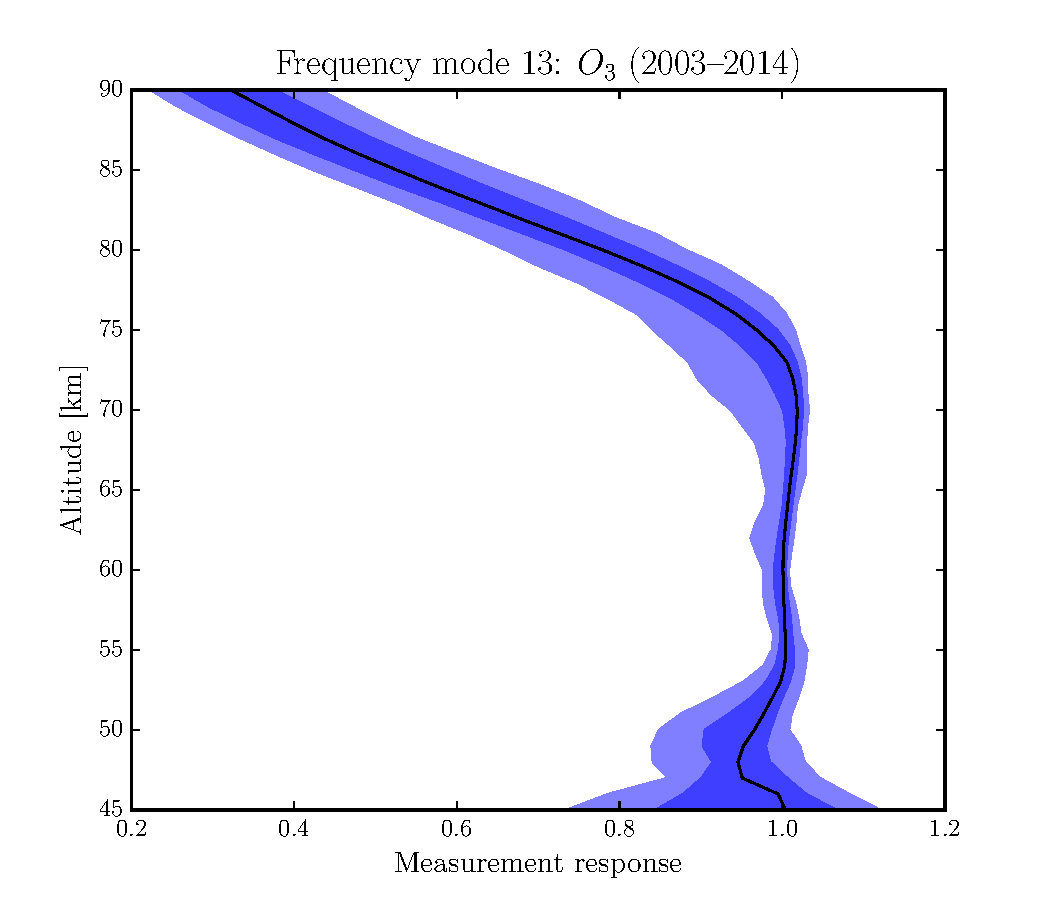
\includegraphics[width=\textwidth]{DDS_fm13_O3_mr}
        \caption{median measurement response with $1\sigma$ and $2\sigma$
        percentiles}
        \label{fig:fm13:O3:mr}
    \end{subfigure}
    \,
    \begin{subfigure}[b]{0.49\textwidth}
        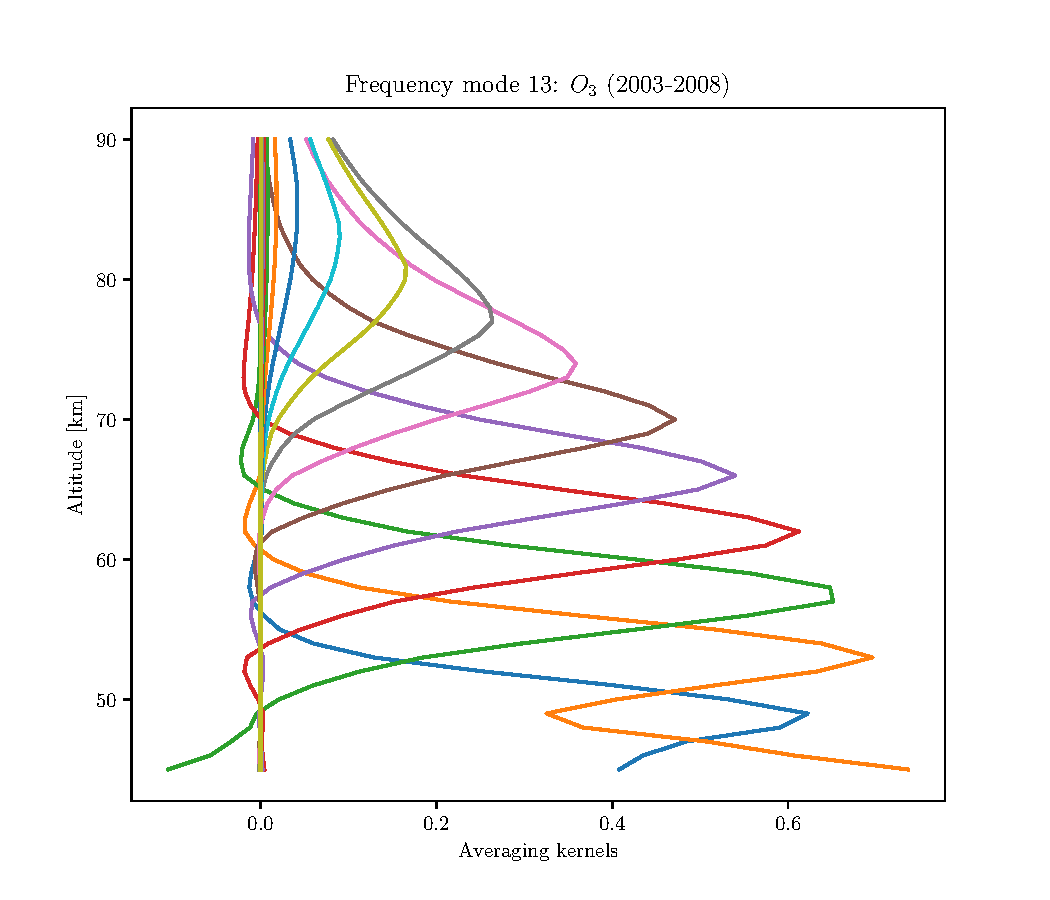
\includegraphics[width=\textwidth]{DDS_fm13_O3_avk}
        \caption{median averaging kernels\newline~}
        \label{fig:fm13:O3:avk}
    \end{subfigure}
    \caption{Measurement response and averaging kernels for \chem{O_3}
    retrievals for \smr~v3 at different altitudes for frequency mode~13.}
    \label{fig:fm13:O3:mr_avk}
\end{figure}


%%%%%%%
% H2O %
%%%%%%%

\subsubsection{\chem{H_2O}}
\label{sec:fm13:comparison:H2O}
The retrievals for \chem{H_2O} have been compared with data from the MIPAS and
MLS instruments. SAGE does not provide reliable water vapour profiles above 33km (\cite{vds}) 
Annual average differences to these instruments are shown in
Figure~\ref{fig:fm13:H2O:profiles}. In Figure~\ref{fig:fm13:H2O:scatter}
individual retrievals for the instruments for the entire period are plotted
against the retrievals from the new and old versions of the \smr\ processing
chain. The results show a slightly improved overall coherency with the
updated version of the processing compared to both considered instruments, but
a systematic under estimation of the concentrations has been introduced, and
the correlation, in particular with MIPAS, remains poor.  This would suggest
that the MIPAS values are  unreliable for this data product. (To be confirmed with KIT)
Figure~\ref{fig:fm13:H2O:mr_avk} suggests that the product is useful over the
range 44--110~km with a vertical resolution of around 4.5~km.


\begin{figure}[tbhp]
    \centering
    \begin{subfigure}[b]{0.49\textwidth}
        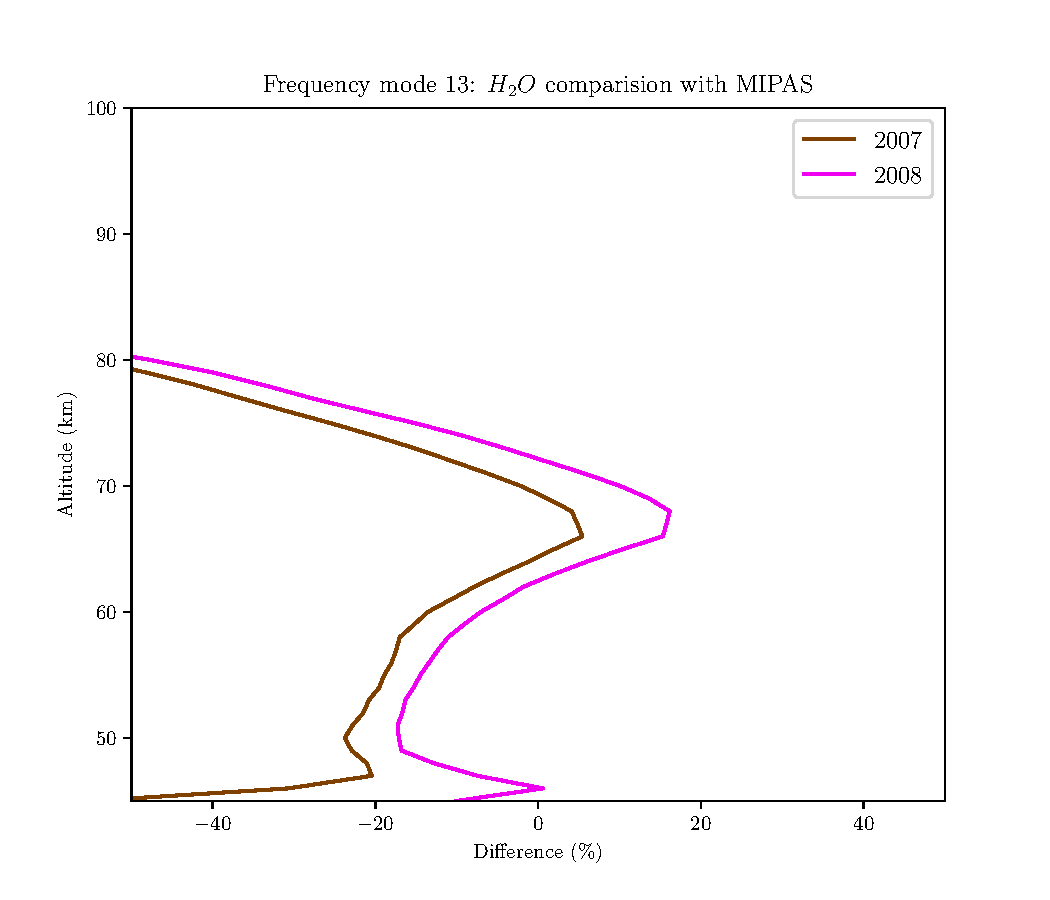
\includegraphics[width=\textwidth]{DDS_fm13_H2O_perdiff_mipas}
        \caption{average difference to MIPAS}
        \label{fig:fm13:H2O:profiles:MIPAS}
    \end{subfigure}
    \,
    \begin{subfigure}[b]{0.49\textwidth}
        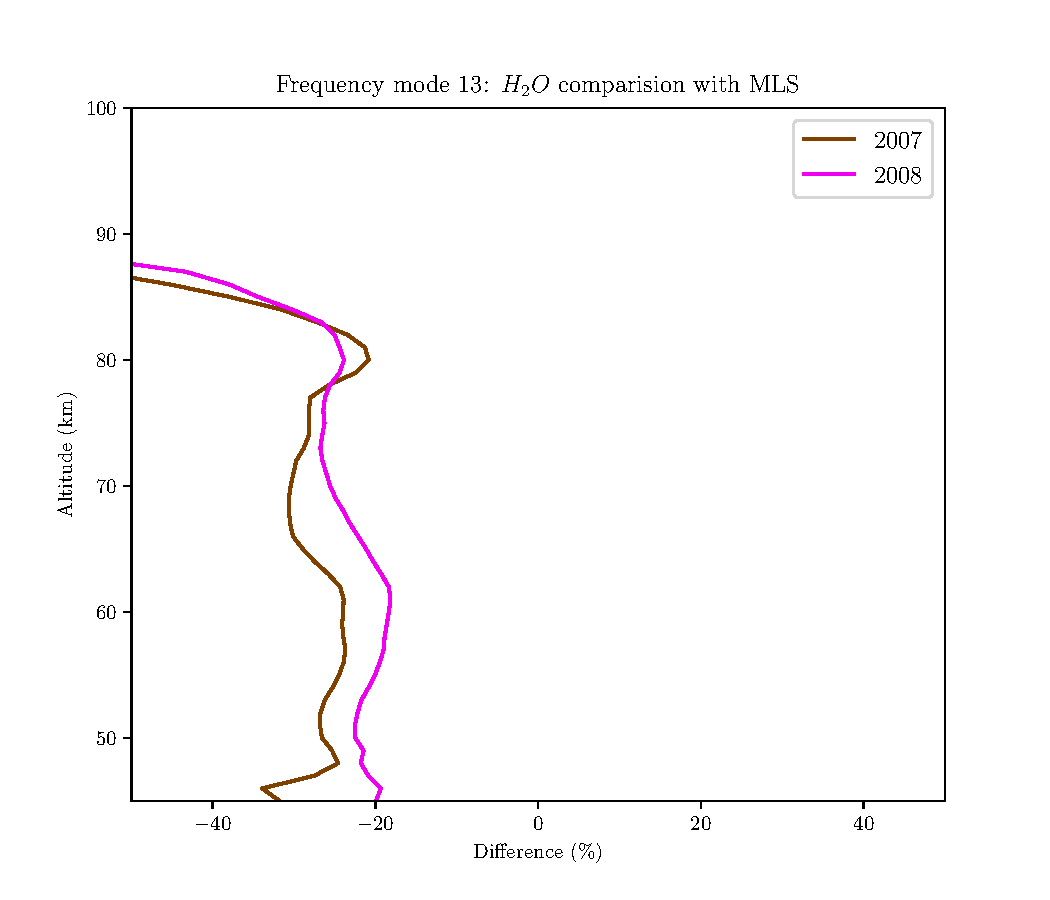
\includegraphics[width=\textwidth]{DDS_fm13_H2O_perdiff_mls}
        \caption{average difference to MLS}
        \label{fig:fm13:H2O:profiles:MLS}
    \end{subfigure}
    \caption{Average difference in percent between retrievals of \chem{H_2O}
    from \smr~v3 and collocated measurements from various instruments at
    different altitudes for frequency mode~13.}

    \label{fig:fm13:H2O:profiles}
\end{figure}

\begin{figure}[tbhp]
    \centering
    \begin{subfigure}[b]{0.49\textwidth}
        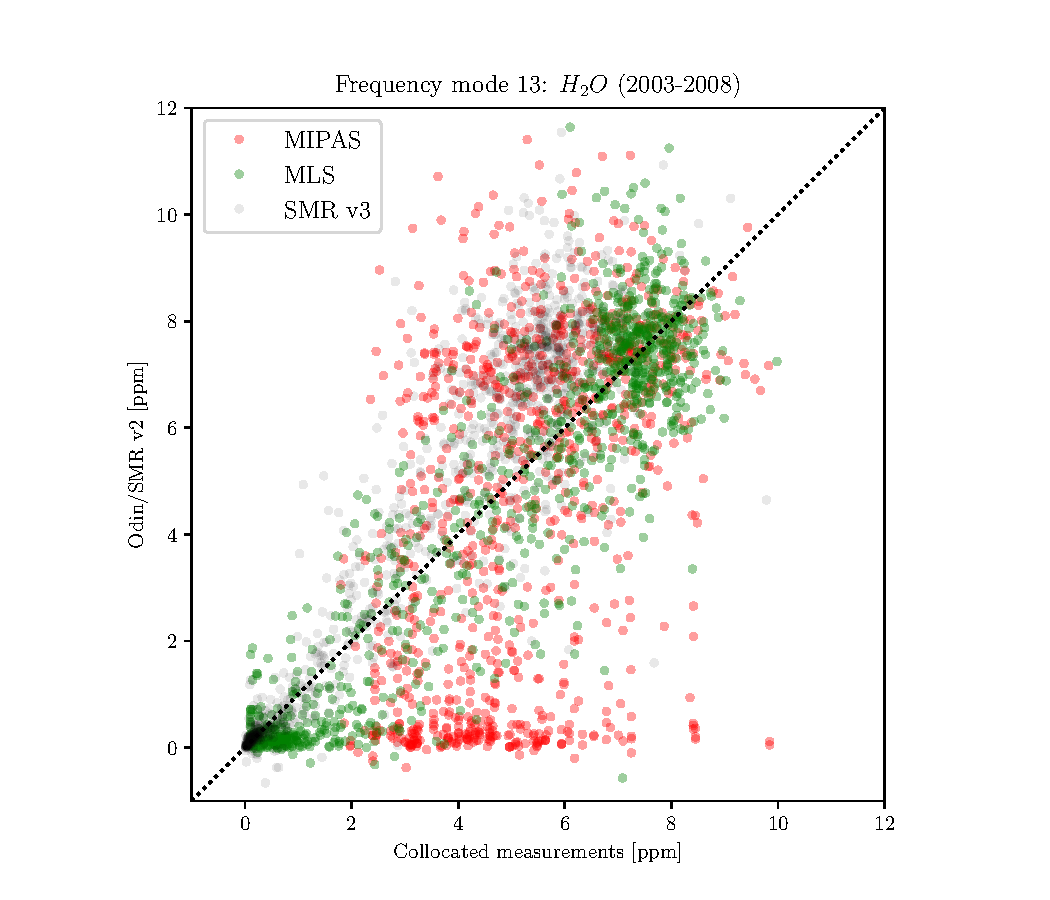
\includegraphics[width=\textwidth]{DDS_fm13_H2O_scatter_v2}
        \caption{correlation of collcated instruments with \smr~v2.X}
        \label{fig:fm13:H2O:scatter:v2}
    \end{subfigure}
    \,
    \begin{subfigure}[b]{0.49\textwidth}
        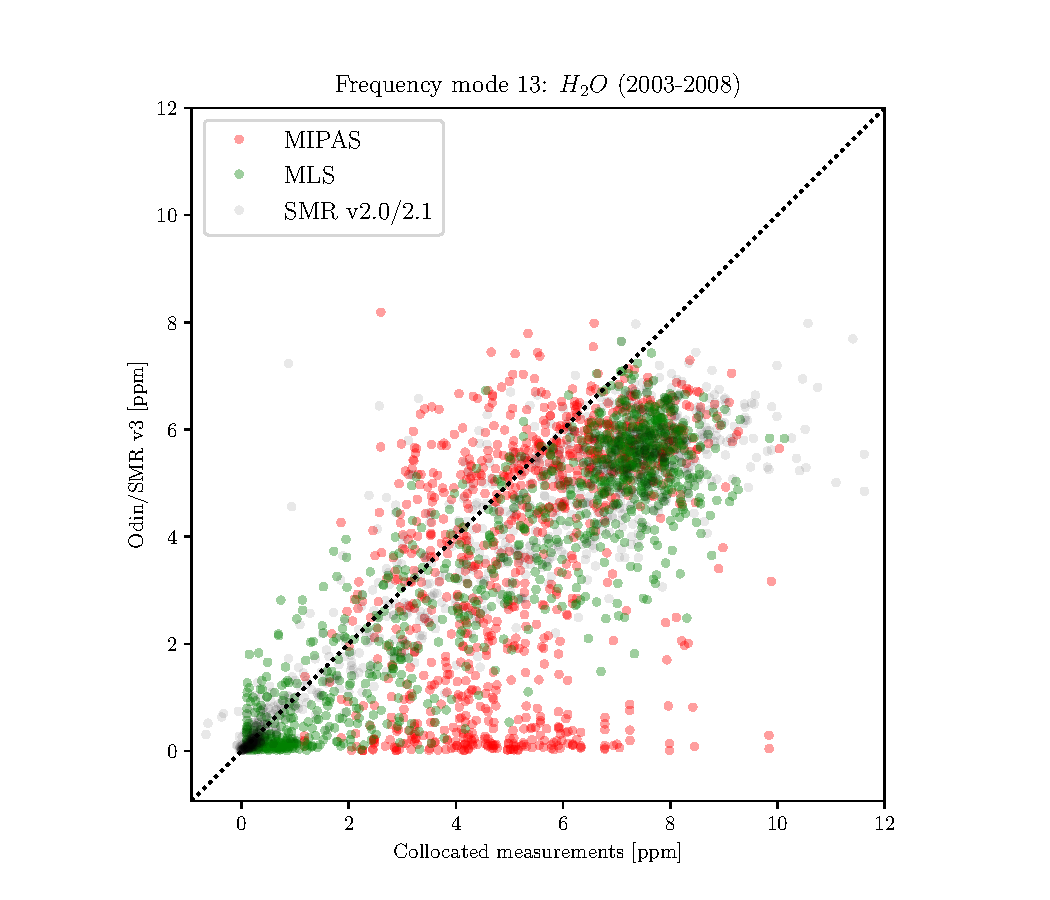
\includegraphics[width=\textwidth]{DDS_fm13_H2O_scatter_v3}
        \caption{correlation of collcated instruments with \smr~v3}
        \label{fig:fm13:H2O:scatter:v3}
    \end{subfigure}
    \caption{Correlation between retrievals of \chem{H_2O} using \smr\
    versions~2.X and~3 and collocated measurements from various instruments
    for frequency mode~13.}
    \label{fig:fm13:H2O:scatter}
\end{figure}

\begin{figure}[tbhp]
    \centering
    \begin{subfigure}[b]{0.49\textwidth}
        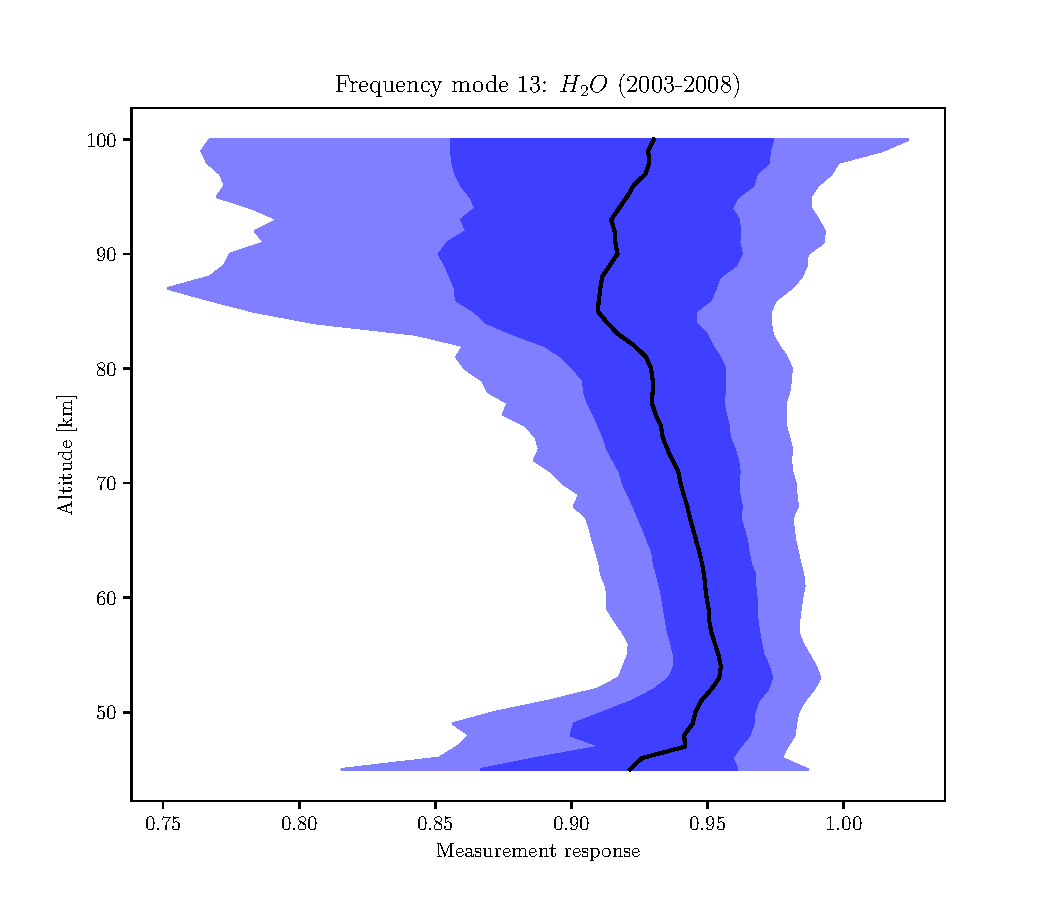
\includegraphics[width=\textwidth]{DDS_fm13_H2O_mr}
        \caption{median measurement response with $1\sigma$ and $2\sigma$
        percentiles}
        \label{fig:fm13:H2O:mr}
    \end{subfigure}
    \,
    \begin{subfigure}[b]{0.49\textwidth}
        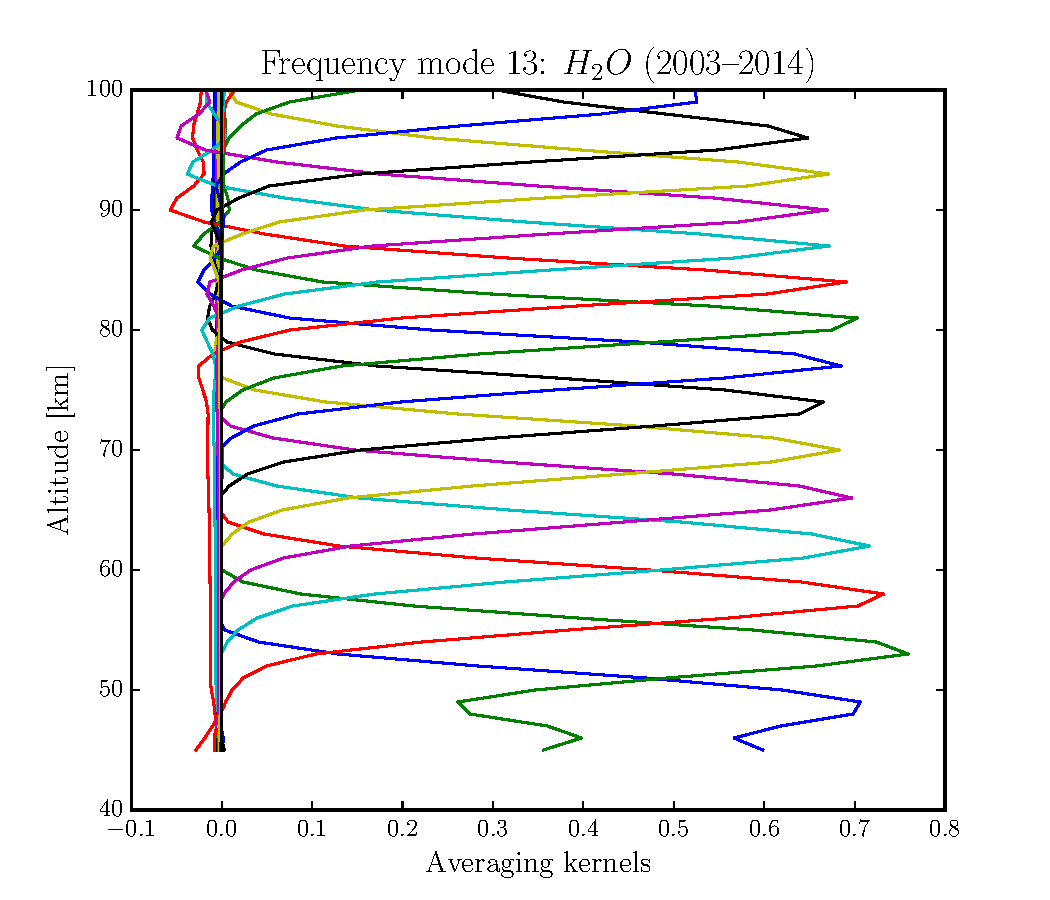
\includegraphics[width=\textwidth]{DDS_fm13_H2O_avk}
        \caption{median averaging kernels\newline~}
        \label{fig:fm13:H2O:avk}
    \end{subfigure}
    \caption{Measurement response and averaging kernels for \chem{H_2O}
    retrievals for \smr~v3 at different altitudes for frequency mode~13.}
    \label{fig:fm13:H2O:mr_avk}
\end{figure}


%%%%%%%%%%%%%%%
% Temperature %
%%%%%%%%%%%%%%%

\subsubsection{\chem{Temperature}}
\label{sec:fm13:comparison:temperature}
The retrievals for temperature have been compared with data from the MLS
instrument. Annual average differences to this instruments are shown in
Figure~\ref{fig:fm13:T:profiles}. In Figure~\ref{fig:fm13:T:scatter} individual
retrievals from MLS for 2003-2014 are plotted against the retrievals
from the new and old versions of the \smr\ processing chain. The results show
little or no improvement with the updated version of the processing. Whereas
with the previous version of the system, the temperature was systematically
over estimated, a small under estimation of the temperature is now seen. This
is a result of the removal of the arbitrary scaling factor.
Figure~\ref{fig:fm13:T:mr_avk} suggests that the product is useful over the
range 44--95~km with a vertical resolution of around 5.5~km.

\begin{figure}[tbhp]
    \centering
    \begin{subfigure}[b]{0.49\textwidth}
        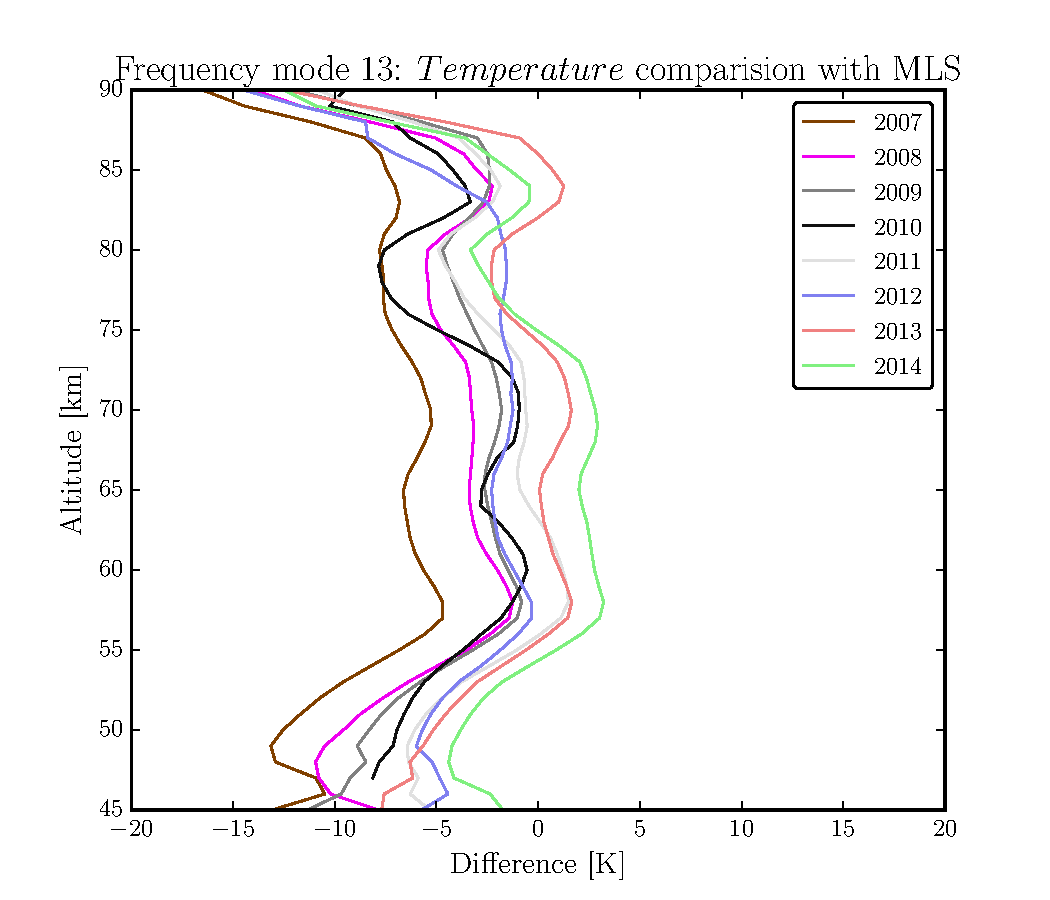
\includegraphics[width=\textwidth]{DDS_fm13_T_absdiff_mls}
        \caption{average difference to MLS}
        \label{fig:fm13:T:profiles:MLS}
    \end{subfigure}
    \caption{Average difference in K between retrievals of temperature from
    \smr~v3 and collocated measurements from MLS at different altitudes.}
    \label{fig:fm13:T:profiles}
\end{figure}

\begin{figure}[tbhp]
    \centering
    \begin{subfigure}[b]{0.49\textwidth}
        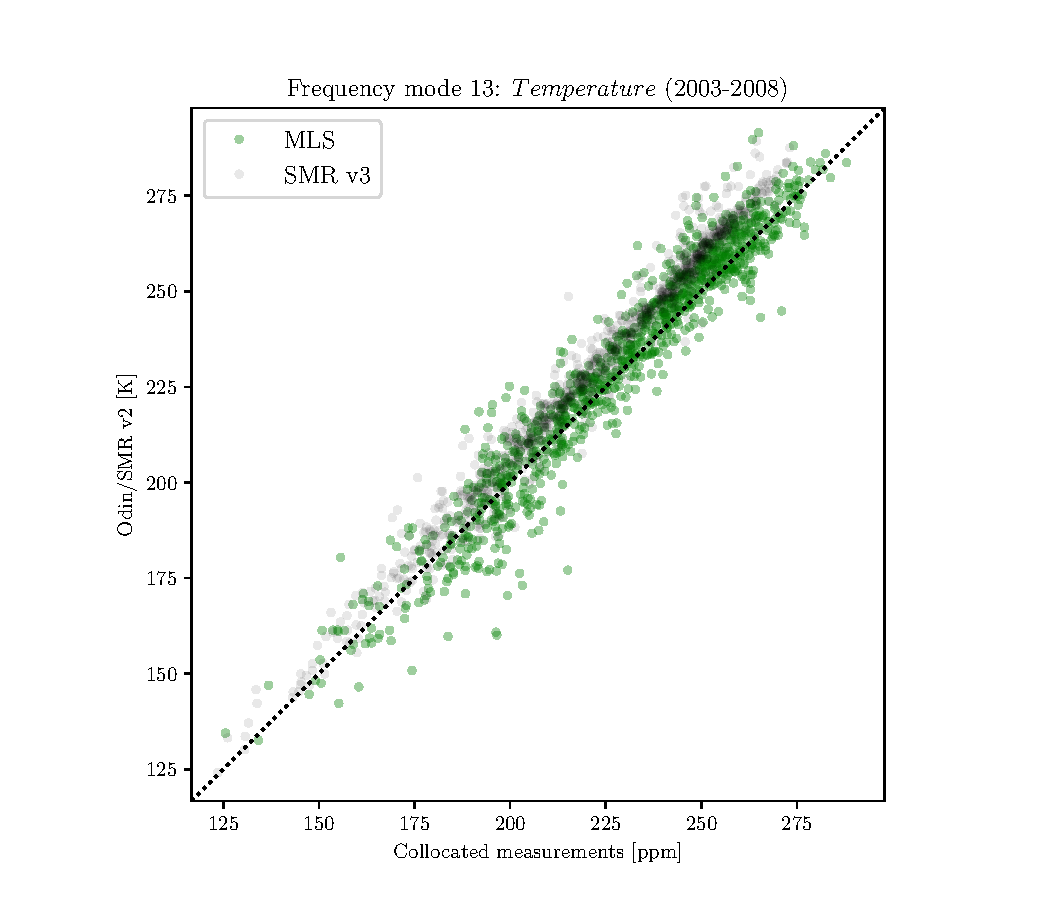
\includegraphics[width=\textwidth]{DDS_fm13_T_scatter_v2}
        \caption{correlation of collcated instruments with \smr~v2.X}
        \label{fig:fm13:T:scatter:v2}
    \end{subfigure}
    \,
    \begin{subfigure}[b]{0.49\textwidth}
        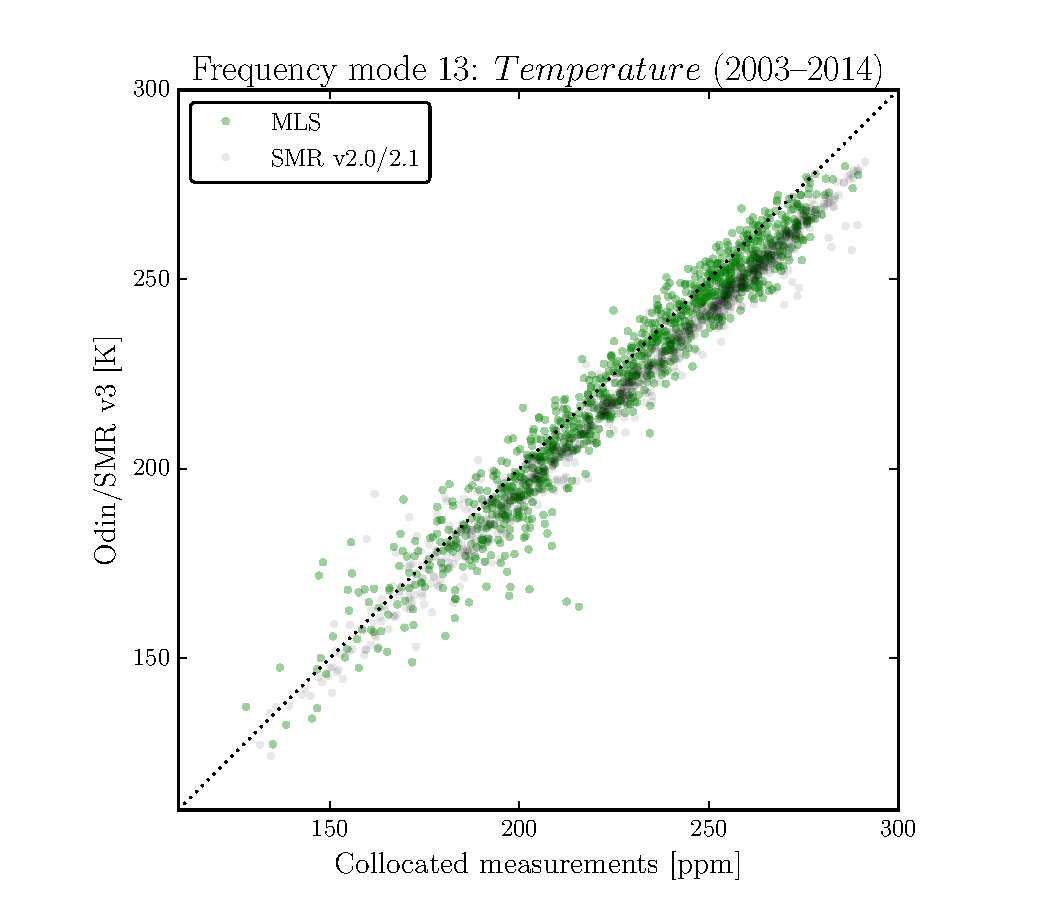
\includegraphics[width=\textwidth]{DDS_fm13_T_scatter_v3}
        \caption{correlation of collcated instruments with \smr~v3}
        \label{fig:fm13:T:scatter:v3}
    \end{subfigure}
    \caption{Correlation between retrievals of temperature using \smr\
    versions~2.X and~3 and collocated measurements from various instruments.}
    \label{fig:fm13:T:scatter}
\end{figure}

\begin{figure}[tbhp]
    \centering
    \begin{subfigure}[b]{0.49\textwidth}
        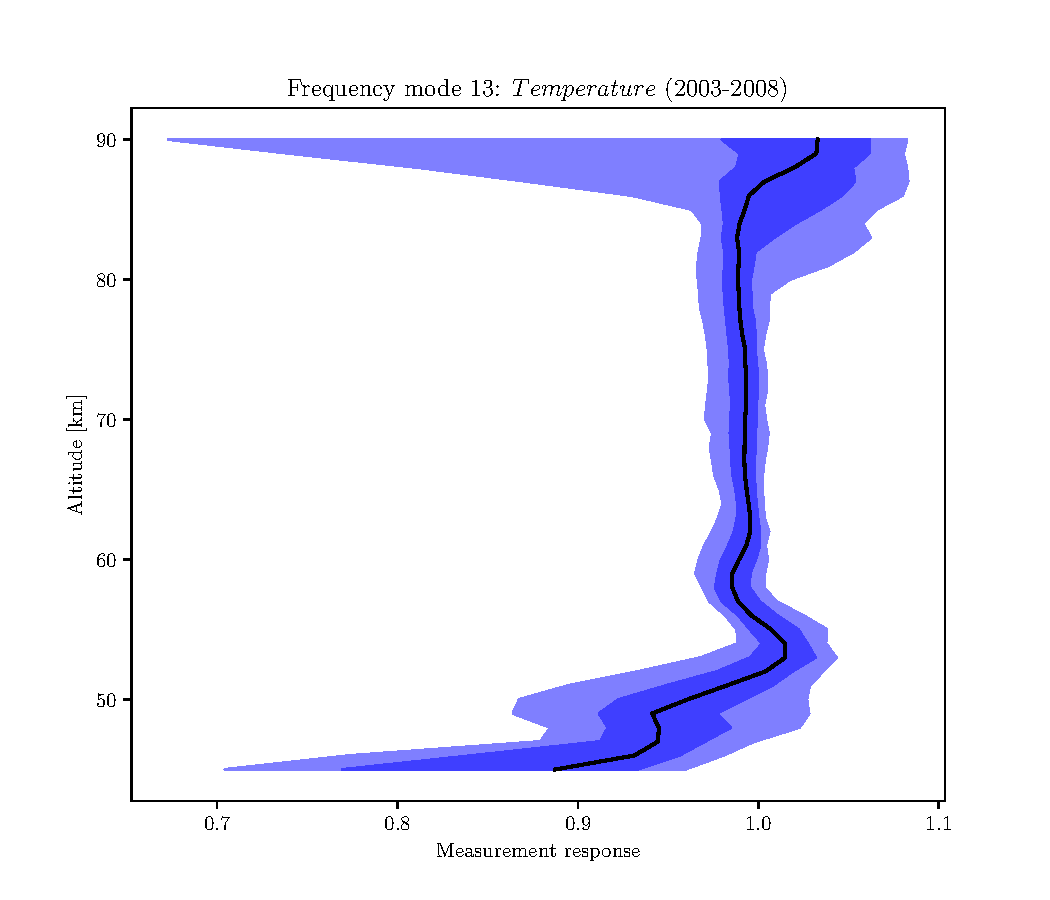
\includegraphics[width=\textwidth]{DDS_fm13_T_mr}
        \caption{median measurement response with $1\sigma$ and $2\sigma$
        percentiles}
        \label{fig:fm13:T:mr}
    \end{subfigure}
    \,
    \begin{subfigure}[b]{0.49\textwidth}
        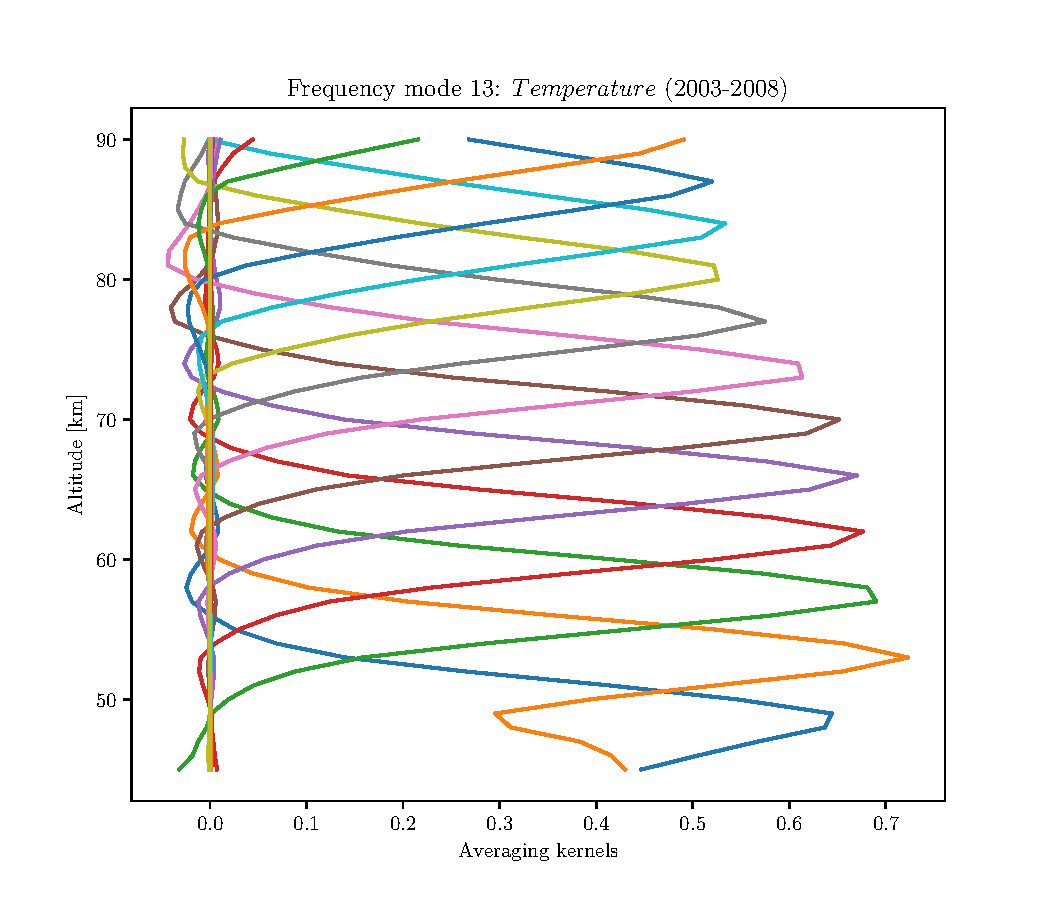
\includegraphics[width=\textwidth]{DDS_fm13_T_avk}
        \caption{median averaging kernels\newline~}
        \label{fig:fm13:T:avk}
    \end{subfigure}
    \caption{Measurement response and averaging kernels for temperature
    retrievals for \smr~v3 at different altitudes for frequency mode~13.}
    \label{fig:fm13:T:mr_avk}
\end{figure}


\subsection{Discussion}
\label{sec:fm13:discussion}
The Pearson correlation between the \smr\ retrievals and the other instruments
was calculated for the entire period for both versions of the processing chain.
The results are summarised in Table~\ref{tab:fm13:stats}, and show that the
new algorithm shows little or no improvement compared to all the instruments
for the species used in this investigation.


\begin{table}[tbhp]
\centering
\caption{Pearson correlation and fit parameters of the old and new \smr\
retrievals for frequency mode~13, compared with collocated data from other
instruments for the period 2003--2014.
}
\label{tab:fm13:stats}
\begin{tabular}{lllrrrr}
    \toprule
    \textbf{Species} & \textbf{Instrument} & \textbf{SMR} & \textbf{corr.} & \textbf{slope} & \textbf{intercept} & \textbf{$\left|\left<\right.\right.$res.$\left.\left.\right>\right|$} \\
    \midrule
    \chem{O3}   & MIPAS     & v3    & 0.795 & 0.757 & 0.026\,ppm    & 0.596\,ppm \\
                &           & v2.x  & 0.687 & 0.827 & 0.185\,ppm    & 0.558\,ppm \\
    \cline{2-7}
                & MLS       & v3    & 0.738 & 0.625 & 0.509\,ppm    & 0.645\,ppm \\
                &           & v2.x  & 0.782 & 0.900 & 0.097\,ppm    & 0.509\,ppm \\
    \cline{2-7}
                & OSIRIS    & v3    & 0.773 & 0.829 & 0.083\,ppm    & 0.461\,ppm \\
                &           & v2.x  & 0.779 & 0.916 & 0.083\,ppm    & 0.355\,ppm \\
    \midrule
    \chem{H_2O} & MIPAS     & v3    & 0.471 & 0.673 & -0.154\,ppm   & 2.924\,ppm \\
                &           & v2.x  & 0.411 & 0.710 & 0.758\,ppm    & 2.965\,ppm \\
    \cline{2-7}
                & MLS       & v3    & 0.890 & 0.776 & -0.134\,ppm   & 1.756\,ppm \\
                &           & v2.x  & 0.877 & 0.940 & -0.224\,ppm   & 1.591\,ppm \\
    \midrule
    Temp.       & MLS       & v3    & 0.959 & 0.986 & -0.250\,K     &  9.090\,K \\
                &           & v2.x  & 0.972 & 1.032 & -4.156\,K     &  8.535\,K \\
    \bottomrule
\end{tabular}
\end{table}

\subsection{Conclusions}
\label{sec:fm13:conclusions}
Based on the discussion above, retrievals based on frequency mode~13 should be
used with caution for both \chem{O_3} and \chem{H_2O}. The temperature
retrievals, on the other hand, appear reliable albeit with a cold bias of
3--5~K. For water vapour he comparisons with MLS seem to suggest a consistent
-20~\% bias.
